%\documentclass[times, utf8, zavrsni]{fer}
%\usepackage{booktabs}
\documentclass[times, utf8, zavrsni, numeric, sort]{fer}
\usepackage{booktabs, url, hyperref}
\usepackage{verbatim}
\usepackage{moreverb}
\usepackage{graphicx}
\usepackage{caption}
\usepackage{subcaption}
\usepackage[space]{grffile}
\usepackage{hyperref}
\usepackage[section,subsection,subsubsection]{extraplaceins}
\usepackage{textcomp}
\usepackage[all]{nowidow}

\hypersetup{
   colorlinks=true,
   citecolor=black,
   filecolor=black,
   linkcolor=black,
   urlcolor=blue
}


\begin{document}


\title{Četvrta laboratorijska vježba}

\author{Davor Cihlar, Tomislav Bošnjak}

\maketitle

\tableofcontents

\chapter{Bijela LED-ica snage 1W}

\section{Uvod}
LED-ice su nelinearni elementi i stoga se napajaju iz strujnog izvora. Kod malih snaga je dovoljan otpornik za ograničenje struje, dok za LED-ice većih snaga takvo rješenje može biti vrlo neefikasno. Korištenjem prekidačkih strujnih izvora umjesto otpornika se mogu postići efikasnosti veće od 90\%.

Ovaj zadatak se sastoji od spajanja prekidačkog strujnog izvora s LED-icom i izvorom napajanja.

Odabrana LED-ica je nazivne snage od 3W (pri 300mA), a interno je izvedena od serijskog i paralelnog spoja nekoliko manjih LED-ica (iz tog razloga odabrana LED-ica počinje raditi tek oko 9V).

LED-icu ćemo napajati s otprilike 1W iako ona može izdržati 3W. Razlog tomu je što se s 3W puno više grije i potreban joj je hladnjak kako temperatura ne bi prešla 80{\textdegree}C (iznad te temperature može doći do oštećenja LED-ice).

Odabrani strujni izvor je baziran na čipu \href{http://www.xlsemi.com/datasheet/XL4001\%20datasheet.pdf}{XL4001} koji kao senzor izlazne struje koristi shunt otpornik (odnosno paralelan spoj tri otpornika -- vidi sliku \ref{fig:leddriverpinout}). XL4001 održava napon od 0.155V na shuntu, što znači da je izlazna struja $I=U/R=0.155/R$.

Podijeljenim strujnim izvorima iz skupne narudžbe su već izvađena dva otpornika tako da je konačan otpor 1$\Omega$ (ili 1.5$\Omega$ -- ovisno o izvedbi) iz čega se može izračunati da je izlazna struja 155mA (ili 103mA).

XL4001 ima mogućnost prigušenja (engl. \textit{dimming}) intenziteta PWM signalom. Tu mogućnost ćemo koristiti pomoću Arduinovog PWM izlaza.

\subsection{Materijali}

\begin{minipage}{1.0\textwidth}

	\begin{itemize}
		\setlength{\itemsep}{0pt}
		\setlength{\parskip}{0pt}

		\item Prekidački strujni izvor $\times$ 1
		\item Bijela LED-ica snage 3W $\times$ 1
		\item Licnate (lako savitljive) žice
	\end{itemize}

	\centering
	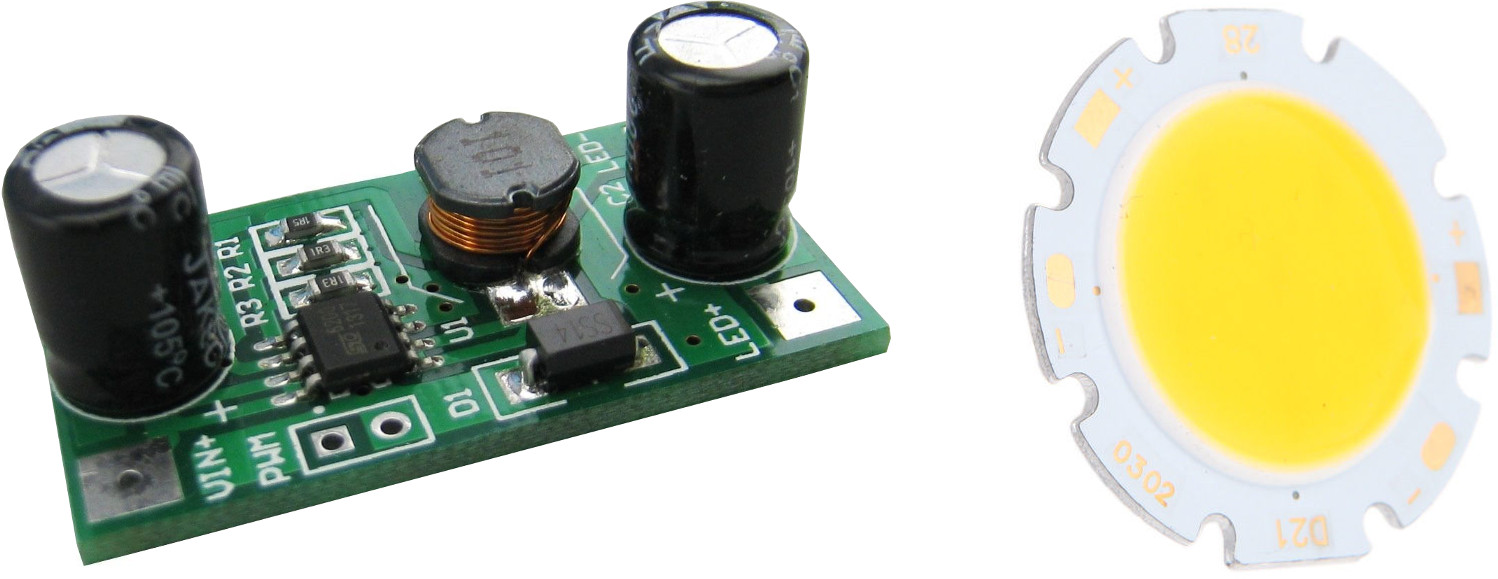
\includegraphics[width=7cm]{./Fotke/1W LED/Materijal.jpg}
	\label{fig:slika1}
\end{minipage}



\subsection{Sklop}

\begin{figure}[htb]
	\centering
	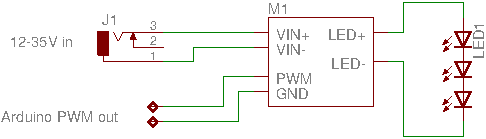
\includegraphics[width=8cm]{./Sklopovi/1W LED/sklop.pdf}
	\caption{Shema sklopa}
	\label{fig:ledshema}
\end{figure}

\begin{figure}[htb]
	\centering
	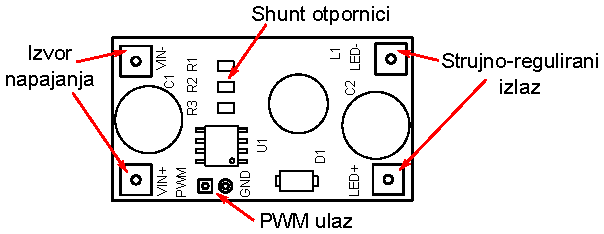
\includegraphics[width=8cm]{./Sklopovi/1W LED/pinout.pdf}
	\caption{Priključci strujnog izvora}
	\label{fig:leddriverpinout}
\end{figure}

\section{Izrada}
\subsection{Osnovni sklop}
Prema shemi na slici \ref{fig:ledshema} spojite izlaze regulatora \texttt{LED+} i \texttt{LED-} na ulaze LED-ice \texttt{+} i \texttt{-}. Zatim zalemite žice na ulaze regulatora \texttt{VIN+} i \texttt{VIN-}. Drugi kraj tih žica će se spajati na izvor napajanja (npr. adapter).

Za sve spojeve je preporučeno koristiti licnate žice kako bi se smanjila mogućnost pucanja na lemnim točkama. Licnate žice, za razliku od krutih, su napravljene od više tankih bakrenih niti.

Ukoliko želite \texttt{VIN+} i \texttt{VIN-} spajati preko eksperimentalne pločice na izvor napajanja onda morate osigurati da je drugi kraj žice krut kako bi se mogao utaknuti u eksperimentalnu pločicu.

\subsection{PWM ulaz}
PWM ulaz (za prigušenje intenziteta) će se spajati na Arduino. Na kontakte PWM ulaza možete zalemiti ili žice ili muški redni konektor ili ženski redni konektor. Odaberite opciju koja vam najviše odgovara.

\subsection{Izmjena izlazne struje}
Ukoliko ste sami naručivali prekidački strujni izvor onda morate izlemiti dva shunt otpornika (poželjno tako da preostane otpornik većeg iznosa). U protivnom (ako ste naručivali skupno) nisu potrebne nikakve dodatne dorade.

Za povećanje izlazne snage zaviriti u poglavlje \ref{sec:powerinc}.

\section{Testiranje}
Na ulaz regulatora (\texttt{VIN+} i \texttt{VIN-}) spojiti naponski izvor (npr. adapter) napona 12V i izmjeriti napon na LED-ici. Izmjereni napon mora biti oko 10V.

Po želji možete provjeriti i ulaznu snagu tako da izmjerite struju iz naponskog izvora i pomnožite ju s odabranim naponom (12V). Očekivana vrijednost je oko 1.5W (ili 1W, ovisno o izvedbi). Za preciznije mjerenje izmjerite i napon dobiven iz izvora jer može odstupati od odabranog (pogotovo ako se radi o klasičnom adapteru s transformatorm).

\section{Moguća poboljšanja}

\subsection{Konektor za izvor napajanja}
Na drugi kraj žica za izvor napajanja (\texttt{VIN+} i \texttt{VIN-}) možete spojiti ženski DC konektor kako bi se adapter mogao direktno na njega priključiti. To bi bilo elegantno rješenje koje minimizira komplikacije oko spajanja na adapter.

\subsection{Povećanje snage}
\label{sec:powerinc}
Ako vam 1W nije dovoljno i želite nazad dobiti 3W morate osigurati hladnjak za LED-icu i SMD otpornike od 1$\Omega$ (moguće i 1.5$\Omega$) dimenzija 0805.

Neprerađeni strujni izvor je kao shunt imao paralelan spoj tri otpornika iznosa 1$\Omega$, 1$\Omega$ i 1.5$\Omega$ što je ukupno iznosilo 375m$\Omega$ i to je vrijednost kojoj se želite približiti na bilo koji način.

Imajte na umu da je za snage veće od 1W potreban adekvatni hladnjak koji može disipirati dovoljno topline da maksimalna temperatura ne prelazi 80{\textdegree}C.


\chapter{Niz upravljivih LED-ica WS2812B}
\section{Uvod}

\href{https://cdn-shop.adafruit.com/datasheets/WS2812B.pdf}{WS2812B} je RGB (engl. \textit{red-green-blue}) LED-ica s ugrađenim upravljačkim integriranim krugom koji omogućuje jednostavnu kontrolu putem namjenskog asinkronog serijskog sučelja.

LED-ice WS2812B je moguće spajati u kaskadu što još dodatno pojednostavljuje cijeli sklop. Primjerice, moguće je spojiti preko 1024 LED-ice na samo jedan GPIO pin bez ikakvog dodatnog sklopovlja. Sve što je jednoj LED-ici potrebno su otpornik za ograničenje struje i blokadni kondenzator (vidi shemu na slici \ref{fig:ws2812b-module}).

Iz tog su razloga ove LED-ice vrlo popularne u dekorativnoj rasvjeti, a moguće ih je koristiti i za velike LED displaye.

\subsection{Materijali}

\begin{figure}[h!]
	\centering
	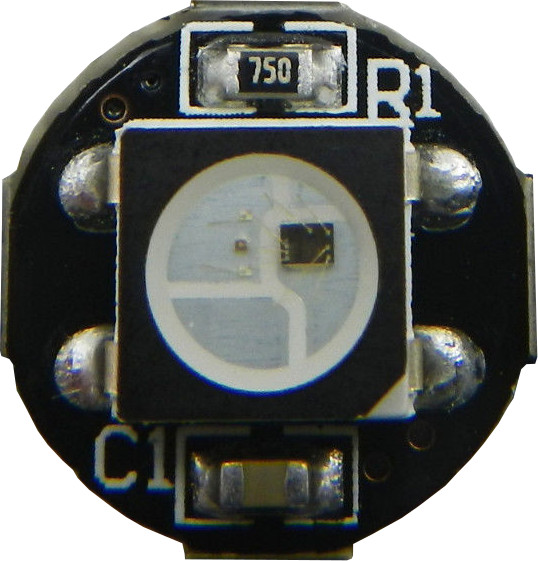
\includegraphics[width=3cm]{./Fotke/WS2812B/Materijal.jpg}
	\label{fig:slika1}
\end{figure}

\begin{itemize}
	\setlength{\itemsep}{0pt}
	\setlength{\parskip}{0pt}
	
	\item Modul s LED-icom WS2812B $\times$ 3
	\item Žice
\end{itemize}

\subsection{Sklop}

\begin{minipage}{1.0\textwidth}
	\centering
	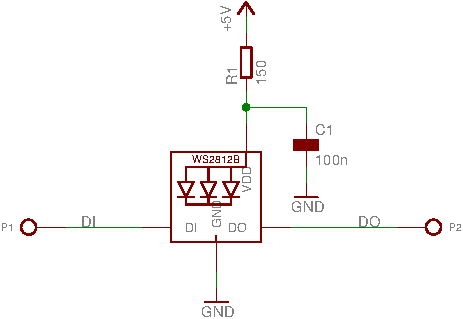
\includegraphics[width=6cm]{./Sklopovi/WS2812B/WS2812B-module.pdf}

	\label{fig:ws2812b-module}
\end{minipage}
\captionof{figure}{Shema jednog modula}

\begin{minipage}{1.0\textwidth}
	\centering
	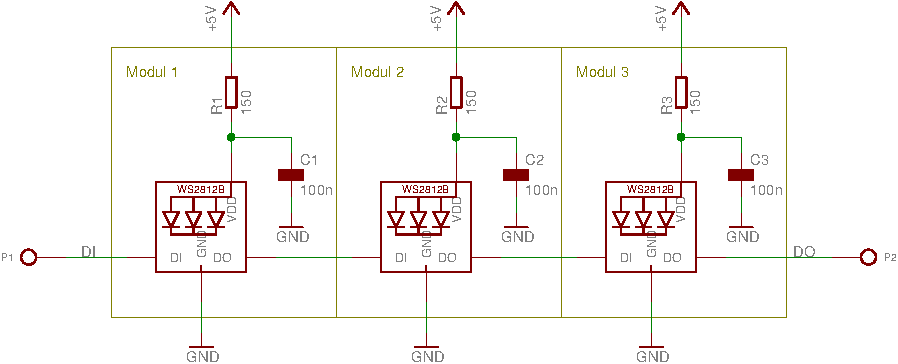
\includegraphics[width=8cm]{./Sklopovi/WS2812B/WS2812B-strip.pdf}
	\label{fig:ws2812b-strip}
\end{minipage}
\captionof{figure}{Shema sklopa}

\section{Izrada}

Nabavljene LED-ice su već zalemljene na pločici zajedno s otpornikom za ograničenje struje i blokadnim kondenzatorom. S donje strane pločice se nalaze lemni kontakti za napajanje i podatkovni signal.

Sve što je potrebno je spojiti tri takva modula u kaskadu prema shemi na slici \ref{fig:ws2812b-strip}. Podatkovni signal se ulančava (izlaz iz LED$_N$ ide na ulaz LED$_{N+1}$), a napajanje se spaja paralelno. Žice iz LED$_1$ če se spajati na Arduino (konkretno na \texttt{GND}, \texttt{+5V} i bilo koji GPIO).


\chapter{Boost regulator napona za 5V}
\section{Uvod}

Brojni elektronički uređaji danas se napajaju pomoću baterija. Problem se u ovom slučaju javlja u naponskim razinama koje baterije daju, te razine koje su potrebne za rad uređaja, poput 3.3 i 5V. Naponi pojedinih baterija kreću se u iznosima 1.2V ili 1.5V (poput alkalnih, NiCd te NiMh punjivih baterija) i 3.6 -- 4.2V za litij-ionske baterije. Željene napone za digitalne elektroničke sklopove moguće je dobiti korištenjem nekog od linearnih regulatora napona koji na sebe preuzmu "višak" napona. Ovo je energetski neefikasno. Drugi način je korištenje prekidačkih izvora napajanja koji su energetski efikasniji od linearnih regulatora.

Prekidački izvori napajanja dijele se na \textit{step-up}, \textit{step-down} i kombinirane izvedbe. U ovom dokumentu govoriti ćemo o \textit{step-up} izvoru napona. On je u slučaju baterijskog napajanja zgodan jer za razliku od \textit{step-down} napajanja imamo manje baterija u seriji kako bi dobili npr. 5V, čime se je postigla ušteda u prostoru i cijeni baterija. 

\subsection{Materijali}

\begin{figure}[h!]
	\centering
	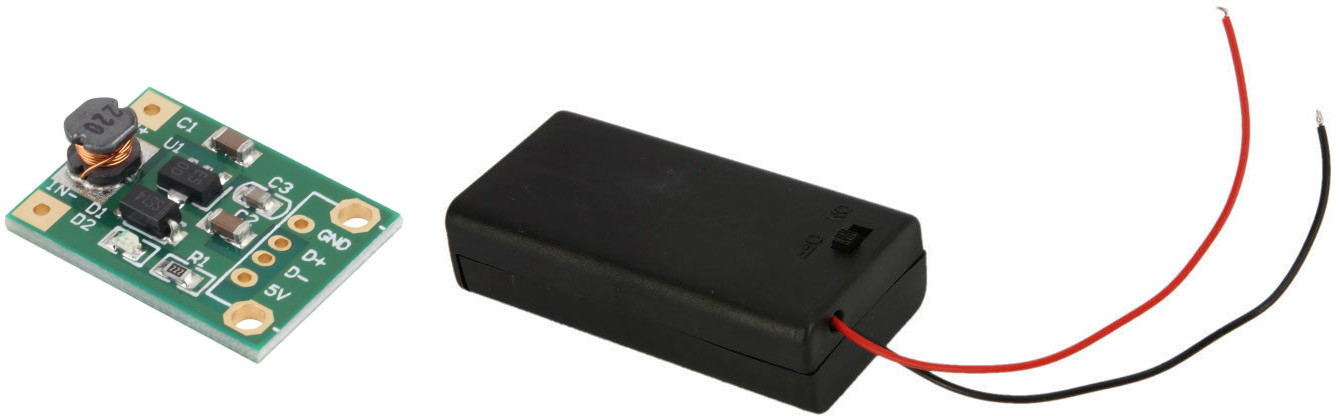
\includegraphics[width=7cm]{./Fotke/5V boost/Materijal.jpg}
	\label{fig:slika1}
\end{figure}

\begin{itemize}
	\setlength{\itemsep}{0pt}
	\setlength{\parskip}{0pt}
	
	\item Prekidački naponski izvor \textit{boost} za 5V $\times$ 1
	\item Kućište za dvije AA baterije s prekidačem $\times$ 1
	\item Žice
\end{itemize}

\subsection{Sklop}

\begin{minipage}{1.0\textwidth}
	\centering
	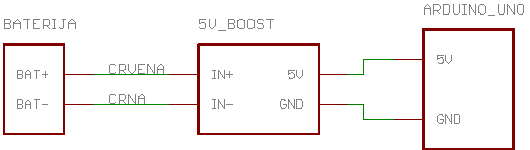
\includegraphics[width=8cm]{./Sklopovi/5V boost/sklop.pdf}
	\label{fig:5Vboost-sch}
\end{minipage}
\captionof{figure}{Shema sklopa}

\begin{minipage}{1.0\textwidth}
	\centering
	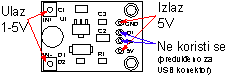
\includegraphics[width=7cm]{./Sklopovi/5V boost/pinout.pdf}
	\label{fig:5Vboost-pinout}
\end{minipage}
\captionof{figure}{Priključci naponskog izvora}

\section{Izrada}
Na ulazne i izlazne priključke zaleme se pinovi (\textit{pin headers}) kako bi se cijela pločica mogla utaknuti u \textit{protoboard}. Naravno, potrebno je paziti da ulazni napon spojimo na odgovarajuće priključke. Ulazni napon dobivamo iz baterija koje su smještene u kućište dobiveno na radionici. Žice iz kućišta leme se na gornju stranu sklopa. Kako bi se spriječio nepotreban utrošak energije baterije u praznom hodu (bez trošila na izlazu napajanja) u kućište je ugrađena sklopka koja galvanski odvaja bateriju od \textit{boost} regulatora.

\section{Testiranje}
Nakon zalemljenih žica iz kućišta na ulaz se spoji napon u rasponu od 1 - 5V te se voltmetrom provjeri da li na izlazu dobivamo 5V. Nakon provjere ispravnog rada možemo testirati napajanje Arduino Uno pločice. Izlazni napon iz našeg \textit{step-up} regulatora spajamo na pinove označene s 5V i GND na \textit{headeru} označenome kao \textit{power}.

\textbf{Napomena:} Dok se koristi ovakav način napajanja Arduino Uno ne smije istodobno biti spojen na druge izvore napajanja (uključujući i računalo preko USB kabela). Time bi istodobno napajali naš sklop iz dva različita izvora čime bi moglo doći do neželjenih struja iz baterije ili USB porta.

\chapter{WiFi modul ESP8266}
\section{Uvod}

WiFi čip s ugrađenim procesorom ESP8266 je po svojem dolasku pokrenuo cijelu lavinu u \textit{communityju} zbog svoje niske cijene i velikih mogućnosti. Iako je originalna dokumentacija na kineskom, ljudi iz \textit{communityja} su ju preveli na engleski što je potom rezultiralo razvojnim okruženjem i integraciji istog u Arduino.

Drugim riječima, moduli bazirani na čipu ESP8266 su vrlo moćni Arduinovi s pristupom na WiFi i cijenom od 2\$. Postoji nekoliko različitih izvedbi modula. Nabavljen je modul ESP-01 koji ima svega 2 dostupna GPIO pina, ali postoje i razni drugi s više GPIO-pinova s više alternativnih funkcija (npr. analogni ulazi).

ESP8266 radi isključivo na 3.3V pa ako se spaja na Arduino mora imati svoj regulator i prilagodbu naponskih razina na TXD i RXD linijama. Cilj ovog zadatka je izraditi noseću pločicu (ESP8266 adapter) s navedenim regulatorom i prilagodbama. Pločica će raditi kao dodatak Arduinu, ali će moći raditi i samostalno -- bez Arduina.

Pločicu će biti moguće utaknuti u eksperimentalnu pločicu zahvaljujući \textit{pin headerima} \texttt{SV1} i \texttt{SV2} (vidi sliku \ref{fig:esp8266-pinout}). Primijetite da su svi pinovi pobrojani po redu kao na čipu i da odgovaraju brojevima pinova u shemi. Takva enumeracija značajno olakšava prepoznavanje uloga pojedinih pinova.

Predviđene su dvije izvedbe pločice: SMD (engl. \textit{Surface Mount Device}) i \textit{through-hole} (standardne velike komponente). Pokušajte izraditi obje varijante kako bi vidjeli razlike u tehnologijama. Na predavanjima se može koristiti bilo koja od te dvije varijante (bitno je samo da je funkcionalna).

\subsection{Materijali}

\begin{figure}[h!]
	\centering
	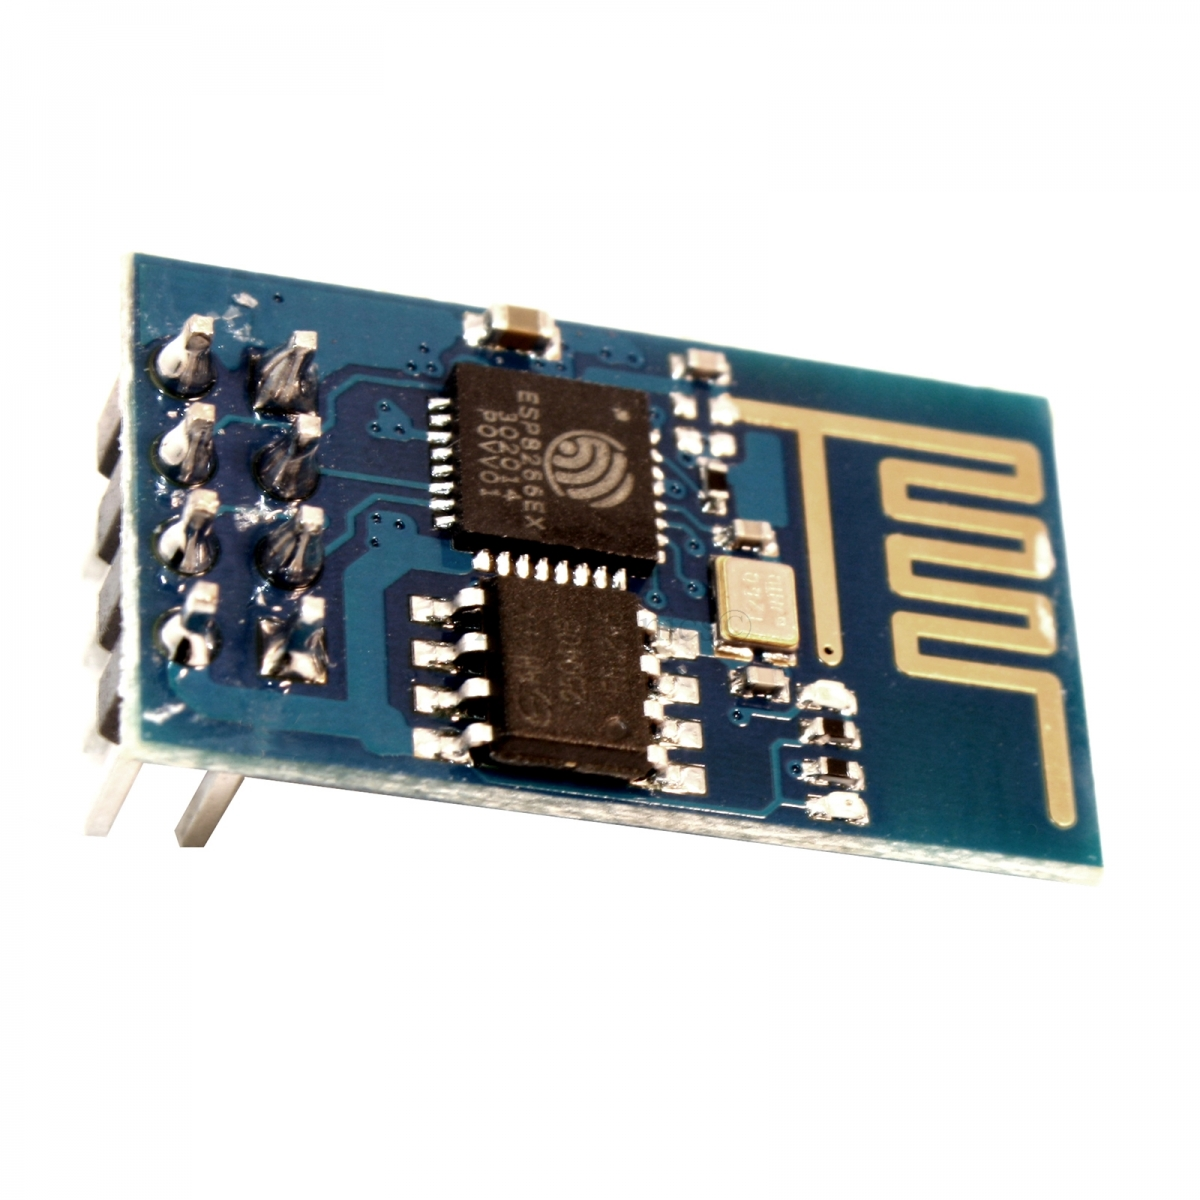
\includegraphics[width=3cm]{./Fotke/ESP8266/Materijal.jpg}
	\label{fig:slika1}
\end{figure}

\begin{itemize}
	\setlength{\itemsep}{0pt}
	\setlength{\parskip}{0pt}
	
	\item Modul ESP-01 $\times$ 1
	\item Adapterska pločica $\times$ 1
	\item Dvoredni konektor ženski, 2$\times$5 priključka $\times$ 1
	\item Redni konektor muški, 5 priključka $\times$ 2
	\item Tantalski kondenzator, 10$\mu$F, 16V $\times$ 1
	\item Tantalski kondenzator, 22$\mu$F, 16V $\times$ 1
	\item Linearni regulator LD1117-33 $\times$ 1
	\item Otpornik 10k$\Omega$ $\times$ 1
	\item Otpornik 15k$\Omega$ $\times$ 1
\end{itemize}

\textbf{Napomena:} Kućište otpornika, kondenzatora i linearnog regulatora ovisi o izvedbi -- SMD ili \textit{through-hole}.

\subsection{Sklop}

\begin{minipage}{1.0\textwidth}
	\centering
	\begin{subfigure}[b]{8cm}
		\centering
		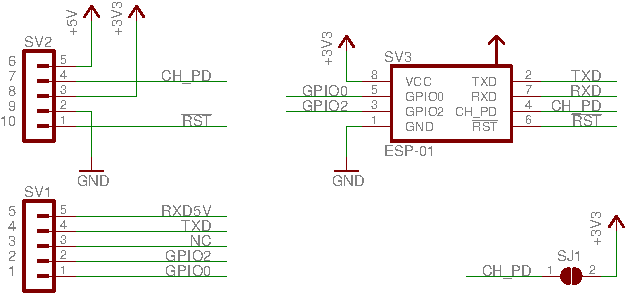
\includegraphics[width=\textwidth]{./Sklopovi/ESP8266/esp8266-adapter-sch-conn.pdf}
		\caption{Konektori}
		\label{fig:esp8266-konektori}
	\end{subfigure}
	\begin{subfigure}[b]{8cm}
		\centering
		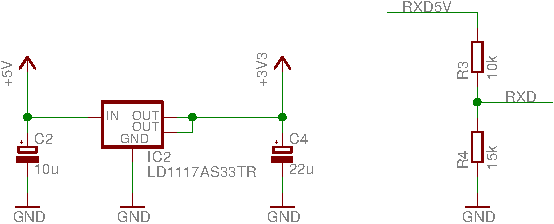
\includegraphics[width=\textwidth]{./Sklopovi/ESP8266/esp8266-adapter-sch-smd.pdf}
		\caption{Varijanta s SMD komponentama}
		\label{fig:esp8266-SMD}
	\end{subfigure}
	\begin{subfigure}[b]{8cm}
		\centering
		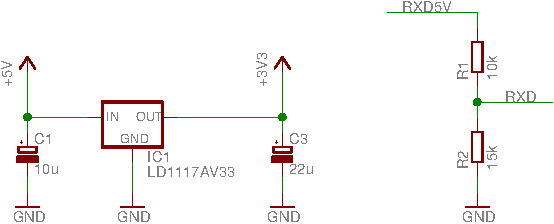
\includegraphics[width=\textwidth]{./Sklopovi/ESP8266/esp8266-adapter-sch-th.pdf}
		\caption{Varijanta s \textit{through-hole} komponentama}
		\label{fig:esp8266-TH}
	\end{subfigure}
\end{minipage}

\begin{figure}[htb]
	\centering
	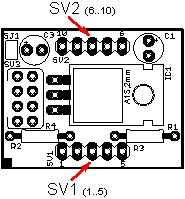
\includegraphics[width=5cm]{./Sklopovi/ESP8266/pinout.pdf}
	\caption{Priključci adaptera}
	\label{fig:esp8266-pinout}
\end{figure}

\section{Izrada}

Izrađuju se dvije varijante pločice -- u SMD tehnologiji i u klasičnoh \textit{through-hole} tehnologiji. Nikako nemojte na istu pločicu zalemiti i SMD i \textit{through-hole} komponente!

\textbf{SMD} varijantu zalemite na prvu pločicu prema shemama na slici \ref{fig:esp8266-konektori} + \ref{fig:esp8266-SMD}.

\textbf{\textit{Through-hole}} varijantu zalemite na drugu pločicu prema shemama na slici \ref{fig:esp8266-konektori} + \ref{fig:esp8266-TH}.

\textbf{U obje varijante} su svi konektori \textit{through-hole} i nužno je pripaziti na koju stranu se leme. \texttt{SV1} i \texttt{SV2} se nalaze na donjoj strani (kako bi se mogli utaknuti u eksperimentalnu pločicu), a \texttt{SV3} se nalazi na gornjoj strani kako bi se u njega mogao utaknuti modul ESP8266.

Prije nego što utaknete modul ESP8266 provjerite da je na pinovima od napajanja (1 i 8 na konektoru \texttt{SV3}) 3.3V kako bi osigurali da nećete uništiti modul previsokim naponom. Potom ugasite napajanje, utaknite modul i nastavite s testiranjem opisanim u idućem poglavlju.

\section{Testiranje}

Arduino će biti korišten u ulozi USB$\rightarrow$serial adaptera za testiranje osnovne funkcionalnosti. Kako MCU ne bi smetao u komunikaciji, potrebno ga je držati pod resetom tako da se spoji \texttt{RST} na \texttt{GND} (u tom modu su svi pinovi u stanju visoke impedancije). Zatim \texttt{RXD} s Arduina treba spojiti na \texttt{RXD} na ESP8266 adapteru i isto tako \texttt{TXD} s Arduina na \texttt{TXD} na adapteru. Nemojte zaboraviti dovesti i napajanje s Arduina na ESP8266 adapter tako da se pinovi \texttt{5V} i \texttt{GND} s Arduina spoje na pinove \texttt{+5V} i \texttt{GND} od ESP8266 adaptera.

Sklop za ispitivanje je sada složen, a ispitivanje kao takvo će se izvoditi u terminalu (Serial Monitor) u grafičkom sučelju Arduino. Stoga priključite Arduino (sklop) na računalo i pokrenite navedeni terminal. Kao terminaciju linije odaberite "Both NL \& CR" te postavite \textit{baud rate} na 9600. Konačno, pošaljite komandu "AT" (bez navodnika) i kao odgovor bi ste trebali dobiti "OK". Ako ne prođe, pokušajte isto na \textit{baud rateu} od 115200.


\chapter{Akcelerometar}
\section{Uvod}

\href{http://www.nxp.com/files/sensors/doc/data_sheet/MMA8452Q.pdf}{MMA8452} je mikroelektromehanički sustav (engl. \textit{MEMS -- Microelectromechanical system}) na čipu za mjerenje akceleracije na tri osi.

Kao sučelje prema mikrokontroleru koristi I$^2$C i može generirati dva različita prekida.

MMA8452Q radi na maksimalno 3.6V, dok Arduino kojeg koristimo radi na 5V tako da nisu direktno kompatibilni. Iz tog razloga je nabavljen modul (pločica s akcelerometrom) koji ima ugrađen naponski regulator za 3.3V te \textit{level-converter} za sabirnicu I$^2$C preko kojeg se MMA8452Q može sigurno spojiti na 5-voltnu logiku.

\subsection{Materijali}
\begin{figure}[h!]
	\centering
	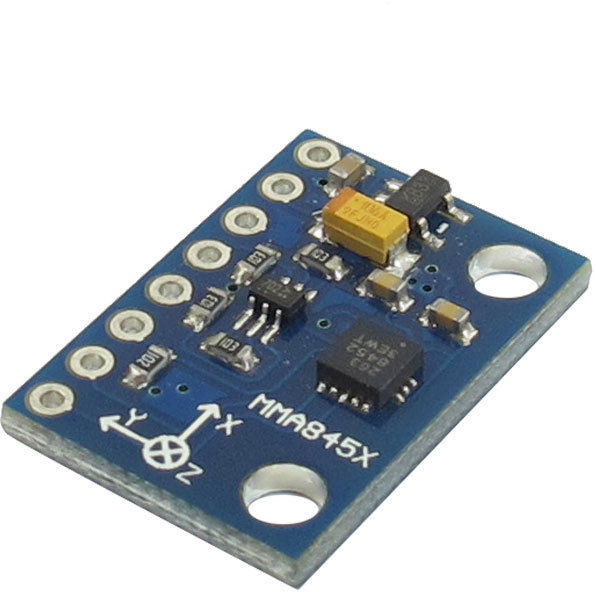
\includegraphics[width=3cm]{./Fotke/MMA8452/Materijal.jpg}
	\label{fig:slika1}
\end{figure}

\begin{itemize}
	\setlength{\itemsep}{0pt}
	\setlength{\parskip}{0pt}
	
	\item Akcelerometar MMA8452 $\times$ 1
	\item Žice
\end{itemize}

\section{Izrada}

Sa stražnje strane modula su navedeni nazivi pojedinih kontakata. Od svih signala biti će korišteni samo \texttt{GND}, \texttt{VCC\_IN}, \texttt{SCL} i \texttt{SDA}, te je stoga samo njih potrebno izvući kako bi se mogli spojiti na Arduino.

Modul će biti korišten zajedno s LED matrix displayem tako da ga je potrebno na neki način pričvrstiti paralelno po svim osima s displayem (nije bitno ako se zamijene neke osi) i žice moraju biti adekvatno duge kako bi se display mogao pomicati bez da se neka od žica odspoji od Arduina.

\end{document}
